\section{算法精度与计算成本}
\label{sec:opt-smooth-accuracy-cost}

前面各节为每个算法给出了各自的保证，但这些保证衡量的对象不同：有的控制目标差，有的控制梯度，有的控制到最小点的距离；有的数迭代轮数，有的只描述进入邻域之后的行为。本节固定同一个优化问题，研究两件事：在同一误差标准下，各方法返回的候选有多准确、为此付出多少工作；以及实际计算中的误差怎样改变这个候选。问题本身的数据变化时最优解怎样移动，是另一类问题，留给下一节。第~\ref{chap:optimization}章已经区分了目标误差、解误差与可计算的残差，并把总成本写成每轮代价与轮数的乘积；本节把这些语言用到光滑优化的具体方法上。

\subsection{收敛速度与总计算成本}
\label{sec:opt-smooth-rates-cost}

\paragraph{三种误差之间的换算}
目标差$f(\bm x)-f^\star$、梯度残差$\lVert\nabla f(\bm x)\rVert_2$和参数误差$\lVert\bm x-\bm x^\star\rVert_2$之间的换算，每个方向都需要自己的条件。

第一，$L$光滑且$f^\star=\inf f>-\infty$时，目标差控制梯度：
\begin{equation}
\label{eq:opt-smooth-gap-controls-gradient}
  \frac1{2L}\lVert\nabla f(\bm x)\rVert_2^2\leq f(\bm x)-f^\star .
\end{equation}
证明只需在式~\eqref{eq:opt-smooth-gd-one-step}中取$\eta=1/L$：$f^\star\leq f(\bm x-\nabla f(\bm x)/L)\leq f(\bm x)-\lVert\nabla f(\bm x)\rVert_2^2/(2L)$。这个方向不需要凸性。

第二，反方向需要曲率的下界。若$f$可微且$\mu$强凸，第~\ref{chap:optimization}章的一阶下界$f(\bm y)\geq f(\bm x)+\langle\nabla f(\bm x),\bm y-\bm x\rangle+\tfrac\mu2\lVert\bm y-\bm x\rVert_2^2$对$\bm y$取最小，右边的最小值是$f(\bm x)-\lVert\nabla f(\bm x)\rVert_2^2/(2\mu)$，于是
\[
  f(\bm x)-f^\star\leq\frac1{2\mu}\lVert\nabla f(\bm x)\rVert_2^2,\qquad\frac\mu2\lVert\bm x-\bm x^\star\rVert_2^2\leq f(\bm x)-f^\star,
\]
后一式是第~\ref{chap:optimization}章强凸误差控制的结论。没有曲率下界时，小梯度不说明小目标差：$f(x)=\tfrac\epsilon2x^2$的梯度是$\epsilon x$，目标差是$\tfrac\epsilon2x^2=g^2/(2\epsilon)$，$\epsilon$很小时梯度为$10^{-3}$的点，目标差可以任意大。

\paragraph{PL条件}
强凸性同时保证了唯一最小点和梯度对目标差的控制。线性收敛其实只需要后一半。设$f$可微且$f^\star=\inf f>-\infty$，若存在$\mu>0$使
\begin{equation}
\label{eq:opt-smooth-pl}
  \frac12\lVert\nabla f(\bm x)\rVert_2^2\geq\mu\bigl(f(\bm x)-f^\star\bigr)\qquad\text{对所有}\ \bm x ,
\end{equation}
就说$f$满足\term{Polyak--Łojasiewicz条件}（PL condition），简称PL条件\cite{karimi2016pl}。它用梯度范数的平方控制目标差。把它与步长$1/L$的单步下降式~\eqref{eq:opt-smooth-gd-one-step}组合：
\[
  f(\bm x^+)-f^\star\leq f(\bm x)-f^\star-\frac1{2L}\lVert\nabla f(\bm x)\rVert_2^2\leq\Bigl(1-\frac\mu L\Bigr)\bigl(f(\bm x)-f^\star\bigr),
\]
所以$L$光滑且满足PL条件时，梯度下降的目标差按$(1-\mu/L)^t$线性收敛。由式~\eqref{eq:opt-smooth-gap-controls-gradient}，PL常数必然满足$\mu\leq L$，收缩因子落在$[0,1)$中。$\mu$强凸的可微函数满足PL条件，反过来不成立。$f(\bm x)=\tfrac12(x_1-x_2)^2$凸但不强凸，最小点构成整条直线$x_1=x_2$，而$\tfrac12\lVert\nabla f\rVert_2^2=(x_1-x_2)^2=2f$，PL条件以$\mu=2$成立；$f(x)=x^2+3\sin^2x$甚至不凸（$f''(\pi/2)=-4$），也满足PL条件\cite{karimi2016pl}。所以PL条件给出目标差的线性速度，却不保证凸性，也不保证唯一的参数解；在多解时，“参数误差”需要改为到解集的距离。

\paragraph{各类保证的汇总}
表~\ref{tab:opt-smooth-rates}按误差对象汇总本章的主要速度结论。同一行内的条件、误差对象与返回点一起构成结论，不能拆开互换；不同行之间也不能排成一个无条件的优劣顺序，例如牛顿法的二次收敛只在局部邻域内成立，而梯度下降的$O(1/T)$是从任意初值出发的全局结论。

\begin{table*}[htbp]
  \centering
  \small
  \begin{tabularx}{\linewidth}{@{}>{\raggedright\arraybackslash}p{0.27\linewidth}>{\raggedright\arraybackslash}X>{\raggedright\arraybackslash}p{0.16\linewidth}>{\raggedright\arraybackslash}p{0.2\linewidth}@{}}
    \toprule
    条件 & 算法与返回点 & 误差对象 & 速度 \\
    \midrule
    $L$光滑，下有界 & 梯度下降（固定步长或回溯），历史最佳点 & 梯度范数 & $\min_{t<T}\lVert\nabla f\rVert_2=O(T^{-1/2})$ \\
    凸，$L$光滑，最小点存在 & 梯度下降，最后一点 & 目标差 & $O(1/T)$ \\
    同上 & Nesterov方法，最后一点 & 目标差 & $O(1/T^2)$ \\
    $L$光滑，PL条件 & 梯度下降$\eta=1/L$，最后一点 & 目标差 & $(1-\mu/L)^T$ \\
    正定二次，谱界已知 & 梯度下降／重球法，最佳参数 & 参数误差 & 因子$\tfrac{\kappa-1}{\kappa+1}$／$\tfrac{\sqrt\kappa-1}{\sqrt\kappa+1}$ \\
    Hessian $M$-Lipschitz，下有界 & 立方正则化，精确模型步 & 新点梯度范数 & $O(\varepsilon^{-3/2})$轮 \\
    非退化最小点的邻域 & 牛顿法／不精确牛顿／完整BFGS & 参数误差或梯度 & 二次／依强迫序列／超线性 \\
    \bottomrule
  \end{tabularx}
  \caption{光滑优化的代表性速度结论。$T$为迭代轮数，$\varepsilon$为梯度容差。最后一行是局部收敛阶，只描述进入邻域之后的行为。}
  \label{tab:opt-smooth-rates}
\end{table*}

\paragraph{每轮代价}
比较方法时，要在同一误差标准下合计全部工作：函数值、梯度、Hessian或Hessian向量积的计算次数，线搜索中被拒绝的试探，线性代数运算，以及存储。对$d$维稠密问题，各方法每轮的主要代价大致如下：梯度下降一次梯度加上线搜索的若干次函数值，存储$O(d)$；重球法与Nesterov方法同样一次梯度，多存一个向量；牛顿法形成Hessian并作Cholesky分解，运算$O(d^3)$、存储$O(d^2)$；Newton--CG若内层做$k$步，代价是$k$次Hessian向量积加$O(kd)$次向量运算，存储$O(d)$；BFGS每轮$O(d^2)$运算与存储；L-BFGS为$O(rd)$。每轮便宜不等于总成本低，轮数少也不等于总成本低，两者必须相乘。

\paragraph{同一问题上的比较}
图~\ref{fig:opt-smooth-convergence-cost}用一个二维非二次目标\cite{math-boyd2004convex}
\[
  f(\bm x)=e^{x_1+3x_2-0.1}+e^{x_1-3x_2-0.1}+e^{-x_1-0.1}
\]
比较三种方法，它的最小点为$(-\tfrac12\ln2,0)^\top$，$f^\star=2\sqrt2e^{-0.1}\approx2.559$。三种方法从$(-1,0.8)^\top$出发，都用$\bar\eta=1$、$\gamma=1/2$、$c=10^{-4}$的回溯，BFGS从$\bm C^{(0)}=\bm I$开始。成本按如下约定计数：每次函数值记$1$，每次梯度记$1$，每次Hessian记$d=2$（相当于用$d$次梯度差分形成它），二维线性代数的运算忽略不计。达到$f-f^\star<10^{-8}$时，梯度下降用了$20$轮、成本$96$；BFGS用了$7$轮、成本$19$；阻尼牛顿法用了$4$轮、成本$18$。按轮数看，牛顿法远远领先；按成本看，它与BFGS相当，因为每轮的Hessian要多付$2$个单位。$d$增大时，牛顿法的Hessian成本按$d$倍、分解按$d^3$增长，BFGS的每轮成本按$d^2$增长，比较结果会随之改变。这个例子只说明比较的方法，不能推广成某种方法普遍更好。

\begin{figure*}[htbp]
  \centering
  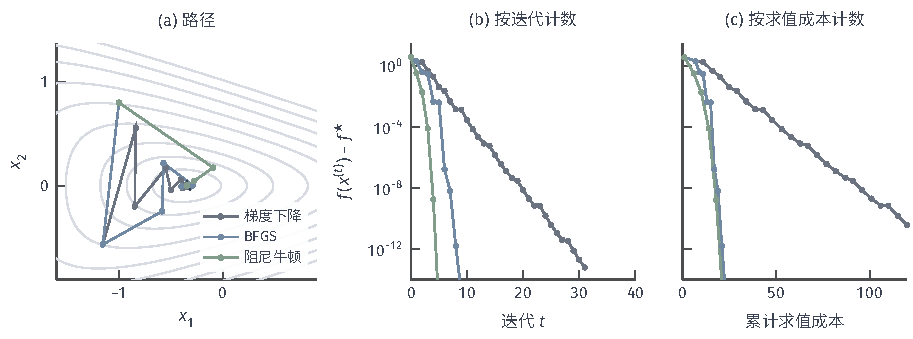
\includegraphics[width=154.6mm]{figures/03-optimization-evolution-and-signals/01-optimization/tikz/c3-convergence-cost/figure.pdf}
  \caption{二维目标$f(\bm x)=e^{x_1+3x_2-0.1}+e^{x_1-3x_2-0.1}+e^{-x_1-0.1}$上三种方法的比较，初值$(-1,0.8)^\top$，均用Armijo回溯（$\bar\eta=1$，$\gamma=1/2$，$c=10^{-4}$）。(a) 等高线上的路径，星号为最小点。(b) 目标差随迭代轮数的变化（对数坐标）：梯度下降（灰）线性下降，BFGS（蓝）后期超线性，阻尼牛顿（绿）最后几步二次收敛。(c) 同一目标差随累计求值成本的变化，函数值与梯度各记$1$，Hessian记$2$；牛顿法与BFGS的差距在这一计数下基本消失。}
  \label{fig:opt-smooth-convergence-cost}
\end{figure*}

在共同例这样的正定二次目标上，比较可以写成公式。梯度下降以最佳固定步长每轮收缩$(\kappa-1)/(\kappa+1)$，把误差缩小到$\varepsilon$倍约需$\tfrac{\kappa}{2}\ln(1/\varepsilon)$轮；重球法约需$\tfrac{\sqrt\kappa}2\ln(1/\varepsilon)$轮，两者每轮都是一次梯度，所以按轮数比较就是按成本比较。$\kappa=10^4$、$\varepsilon=10^{-6}$时，前者约$6.9\times10^4$轮，后者约$690$轮。牛顿法在二次目标上一步到达，但这一步解的线性方程，本身就是原问题。

\subsection{计算误差的传播}
\label{sec:opt-smooth-error-propagation}

到目前为止，每一步都被当作精确执行。实际计算中，梯度可能只是近似值（例如由有限差分或截断的内层迭代得到），求出的位移可能不精确，位移加到参数上时还有舍入。这些误差不会让上一小节的结论完全失效，但会改变可以达到的精度。

\paragraph{误差进入单步下降式}
把实际执行的更新写成
\[
  \tilde{\bm x}^{(t+1)}=\tilde{\bm x}^{(t)}-\eta\bigl(\nabla f(\tilde{\bm x}^{(t)})+\bm e^{(t)}\bigr)+\bm u^{(t)},
\]
其中$\bm e^{(t)}$是方向中的误差（梯度误差或内层求步误差），$\bm u^{(t)}$是位移叠加时的舍入。两者可以合并为有效误差$\bm e_{\mathrm{eff}}^{(t)}=\bm e^{(t)}-\bm u^{(t)}/\eta$，于是实际更新就是带误差$\bm e_{\mathrm{eff}}^{(t)}$的梯度步。设$f$为$L$光滑，$0<\eta\leq1/L$。记$\bm g=\nabla f(\tilde{\bm x}^{(t)})$，$\bm d=\bm g+\bm e_{\mathrm{eff}}^{(t)}$，由下降引理与$L\eta\leq1$，
\[
  f(\tilde{\bm x}^{(t+1)})\leq f(\tilde{\bm x}^{(t)})-\eta\langle\bm g,\bm d\rangle+\frac\eta2\lVert\bm d\rVert_2^2
  =f(\tilde{\bm x}^{(t)})-\frac\eta2\lVert\bm g\rVert_2^2+\frac\eta2\lVert\bm d-\bm g\rVert_2^2,
\]
最后一步是配方$\lVert\bm d\rVert_2^2-2\langle\bm g,\bm d\rangle=\lVert\bm d-\bm g\rVert_2^2-\lVert\bm g\rVert_2^2$。也就是
\begin{equation}
\label{eq:opt-smooth-inexact-step}
  f(\tilde{\bm x}^{(t+1)})\leq f(\tilde{\bm x}^{(t)})-\frac\eta2\lVert\nabla f(\tilde{\bm x}^{(t)})\rVert_2^2+\frac\eta2\lVert\bm e_{\mathrm{eff}}^{(t)}\rVert_2^2 .
\end{equation}
只有当梯度大于误差时，这一步才保证下降。若$f$下有界，按定理~\ref{thm:opt-smooth-gd-nonconvex}的方式累加：
\[
  \min_{0\leq t<T}\lVert\nabla f(\tilde{\bm x}^{(t)})\rVert_2^2\leq\frac{2\bigl(f(\tilde{\bm x}^{(0)})-f_{\inf}\bigr)}{T\eta}+\frac1T\sum_{t=0}^{T-1}\lVert\bm e_{\mathrm{eff}}^{(t)}\rVert_2^2 .
\]
第一项随$T$衰减，第二项是误差的平均，不随$T$消失。误差有一致上界$\epsilon$时，可以保证的梯度残差停在$\epsilon$的量级。

\paragraph{误差下限}
这个下限是真实存在的，不是证明的松弛。取$f(x)=\tfrac12x^2$，$\eta=1/2$，每步的梯度都带有同号的误差$e$：更新$x^+=x-\tfrac12(x+e)$的不动点是$x=-e$，目标停在$e^2/2$。图~\ref{fig:opt-smooth-error-propagation}(a)中，$e=0$时目标几何下降，$e=10^{-2}$与$e=10^{-1}$时分别停在$5\times10^{-5}$与$5\times10^{-3}$附近。

\paragraph{步长越小未必越准}
有效误差中的$-\bm u^{(t)}/\eta$说明，缩小步长会放大舍入误差的相对作用。浮点数加法$x+\delta$在$|\delta|$小于$x$的单位舍入量的一半左右时结果仍是$x$：单精度的单位舍入约$6\times10^{-8}$，若$x_i\approx1$而位移分量$\eta g_i\approx10^{-8}$，这一步在该坐标上完全丢失。梯度误差$\bm e^{(t)}$不随$\eta$变化，舍入项却随$\eta$变小而变大，所以不能笼统地说“步长越小越准确”；缩步只改变不同误差项的相对大小。函数值同样有计算误差：若函数值误差不超过$\tau_f$，Armijo检验通过时真实下降只能保证到计算下降减去$2\tau_f$；梯度误差不超过$\tau_g$时，算出$\lVert\hat{\bm g}\rVert_2\leq\varepsilon$只能推出$\lVert\nabla f\rVert_2\leq\varepsilon+\tau_g$。停止容差小于这些计算误差时，停止判断就不可靠了。

\paragraph{实际轨迹与理想轨迹}
另一个问题是：实际迭代与精确执行的迭代相差多远，前面混入的误差会衰减、积累还是放大？记理想更新映射$T(\bm x)=\bm x-\eta\nabla f(\bm x)$，若它满足$\lVert T(\bm x)-T(\bm y)\rVert_2\leq q\lVert\bm x-\bm y\rVert_2$，则理想轨迹$\bm x^{(t)}$与实际轨迹$\tilde{\bm x}^{(t)}$的偏差$\delta^{(t)}=\lVert\tilde{\bm x}^{(t)}-\bm x^{(t)}\rVert_2$满足
\[
  \delta^{(t+1)}\leq\lVert T(\tilde{\bm x}^{(t)})-T(\bm x^{(t)})\rVert_2+\eta\lVert\bm e^{(t)}\rVert_2+\lVert\bm u^{(t)}\rVert_2\leq q\,\delta^{(t)}+a^{(t)},
\]
其中$a^{(t)}=\eta\lVert\bm e^{(t)}\rVert_2+\lVert\bm u^{(t)}\rVert_2$是第$t$步新注入的误差。展开得
\begin{equation}
\label{eq:opt-smooth-deviation}
  \delta^{(T)}\leq q^T\delta^{(0)}+\sum_{t=0}^{T-1}q^{T-1-t}a^{(t)} .
\end{equation}
$q<1$时旧误差几何衰减，每步注入$a$时偏差不超过$a/(1-q)$；$q=1$时旧误差不衰减，注入的误差线性积累；$q>1$时早期的误差被指数放大。图~\ref{fig:opt-smooth-error-propagation}(b)以$a=10^{-3}$画出这三种情形，它们分别对应$f(x)=\tfrac\lambda2x^2$、$\eta=1/2$下的$\lambda=0.2$、$0$、$-0.1$，即强凸、平坦与负曲率三种局部形状。

\begin{figure}[htbp]
  \centering
  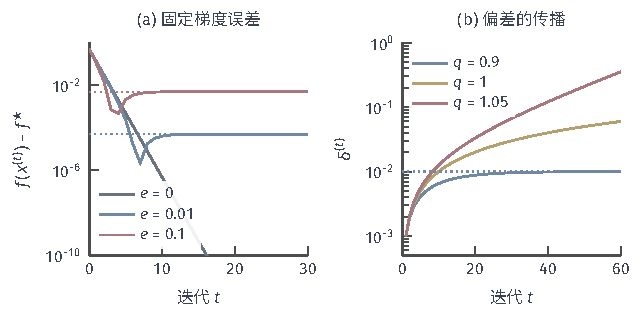
\includegraphics[width=108.5mm]{figures/03-optimization-evolution-and-signals/01-optimization/tikz/c3-error-propagation/figure.pdf}
  \caption{计算误差的影响。(a) $f(x)=x^2/2$上$\eta=1/2$、$x^{(0)}=1$的梯度下降，每步梯度带固定误差$e$；$e>0$时目标停在点线所示的$e^2/2$。(b) 递推$\delta^{(t+1)}=q\,\delta^{(t)}+10^{-3}$的解：$q=0.9$时趋于$0.01$（点线），$q=1$时线性增长，$q=1.05$时指数增长。}
  \label{fig:opt-smooth-error-propagation}
\end{figure}

\paragraph{传播系数从哪里来}
系数$q$由目标的曲率决定。设$f$二阶连续可微，则$T(\bm x)-T(\bm y)=(\bm I-\eta\bar{\bm H})(\bm x-\bm y)$，其中$\bar{\bm H}=\int_0^1\nabla^2f(\bm y+s(\bm x-\bm y))\,\mathrm ds$是线段上的平均Hessian。若沿途$\mu\bm I\preceq\nabla^2f\preceq L\bm I$，则$\bar{\bm H}$的特征值也在$[\mu,L]$中，
\[
  q\leq\max\{|1-\eta\mu|,\ |1-\eta L|\}.
\]
强凸（$\mu>0$）且$0<\eta<2/L$时$q<1$，更新映射是压缩映射；仅凸（$\mu=0$）且$0<\eta\leq2/L$时只有$q\leq1$，误差不衰减；一般的$L$光滑目标只能保证$q\leq1+\eta L$，负曲率方向上偏差会被放大。步长变化时要检查乘积$\prod_t q^{(t)}$，而不是每一项：逐项小于$1$不足以让旧误差消失，例如$q^{(t)}=1-1/(t+2)^2$时乘积趋于$1/2$。

带动量的方法要比较完整的状态。重球法的状态是$(\bm x^{(t)},\bm x^{(t-1)})$，在二次目标上状态按一个$2\times2$分块矩阵演化；这个矩阵的谱半径小于$1$保证误差最终衰减，但它不是对称矩阵，其范数可能大于$1$，偏差在衰减之前可以先短暂增长。两条轨迹即使当前参数$\bm x^{(t)}$相同，只要上一步的位移不同，下一步也会不同。本节只比较离散迭代之间的偏差；把迭代看成连续梯度流$\dot{\bm x}=-\nabla f(\bm x)$的离散化，并研究两者之间的误差，属于本卷第~\ref{part:dynamical-systems-control-decision-and-games}部分“过程与轨迹演化”的内容。
